\chapter{Produto Escalar}

\begin{df} Chama-se produto escalar (ou produto interno usual) de dois vetores $\vec u$ e $\vec v$ o número real representado por $\vec u \cdot \vec v$ ou $<\vec u, \vec v>$ e calculado pela soma dos produtos das componentes correspondentes dos vetores.

No plano, $\mathbb{R}^2$, se $\vec u=(x_1, y_1)$ e $\vec v=(x_2, y_2)$ então $\vec u \cdot \vec v = x_1\cdot x_2 + y_1\cdot y_2$.

No espaço, $\mathbb{R}^3$, se $\vec u=(x_1, y_1, z_1)$ e $\vec v=(x_2, y_2, z_2)$ então $\vec u \cdot \vec v = x_1\cdot x_2 + y_1\cdot y_2+z_1\cdot z_2$.
\end{df}


\section{Propriedades do produto escalar}

\begin{enumerate}[(1)]
\item $\vec u\cdot \vec v=\vec v\cdot \vec u$
\item $\vec u\cdot (\vec v+\vec w)=\vec u\cdot \vec v+\vec u\cdot \vec w$
\item $\alpha(\vec u\cdot \vec v)=(\alpha \vec u)\cdot \vec v=\vec u\cdot (\alpha \vec v)$, com $\alpha \in \mathbb{R}$.
\item $\vec u\cdot \vec u=\Vert \vec u \Vert^2$
\item $\Vert \vec u\cdot \vec v\Vert \leq \Vert \vec u \Vert \Vert \vec v \Vert$ (Desigualdade de Schwarz)
\item $\Vert \vec u + \vec v\Vert \leq \Vert \vec u \Vert+ \Vert \vec v \Vert$ (Desigualdade Triangular)
\end{enumerate}

\subsection{Ângulo entre dois vetores}

Note que quando realizamos o produto escalar entre dois vetores, obtemos um número e que a definição na sua primeira forma nos dá informação sobre o ângulo entre os dois vetores, pois $$\cos{\theta}=\frac{\vec{u} \cdot \vec{v}}{\Vert\vec{u}\Vert \cdot \Vert\vec{v}\Vert}$$

\noindent onde $\theta$ é o ângulo entre os vetores com $0\leq \theta \leq \pi$. A demonstração deste fato pode ser obtida com a utilização da lei dos cossenos e de algumas propriedades (veja bibliografia específica indica.)

Com isso obtemos outra maneira de definir o produto escalar: $$\vec u \cdot \vec v=\Vert \vec u \Vert \cdot \Vert \vec v \Vert \cdot \cos{\theta}$$

Observação: da fórmula acima podemos ver que o sinal de $\vec{u} \cdot \vec{v}$ é o mesmo que o sinal de $\cos{\theta}$ e a partir daí, concluir se o ângulo entre os dois vetores é agudo, obtuso ou reto (vetores ortogonais).

\begin{figure}[H]
\begin{minipage}[b]{0.3\linewidth}
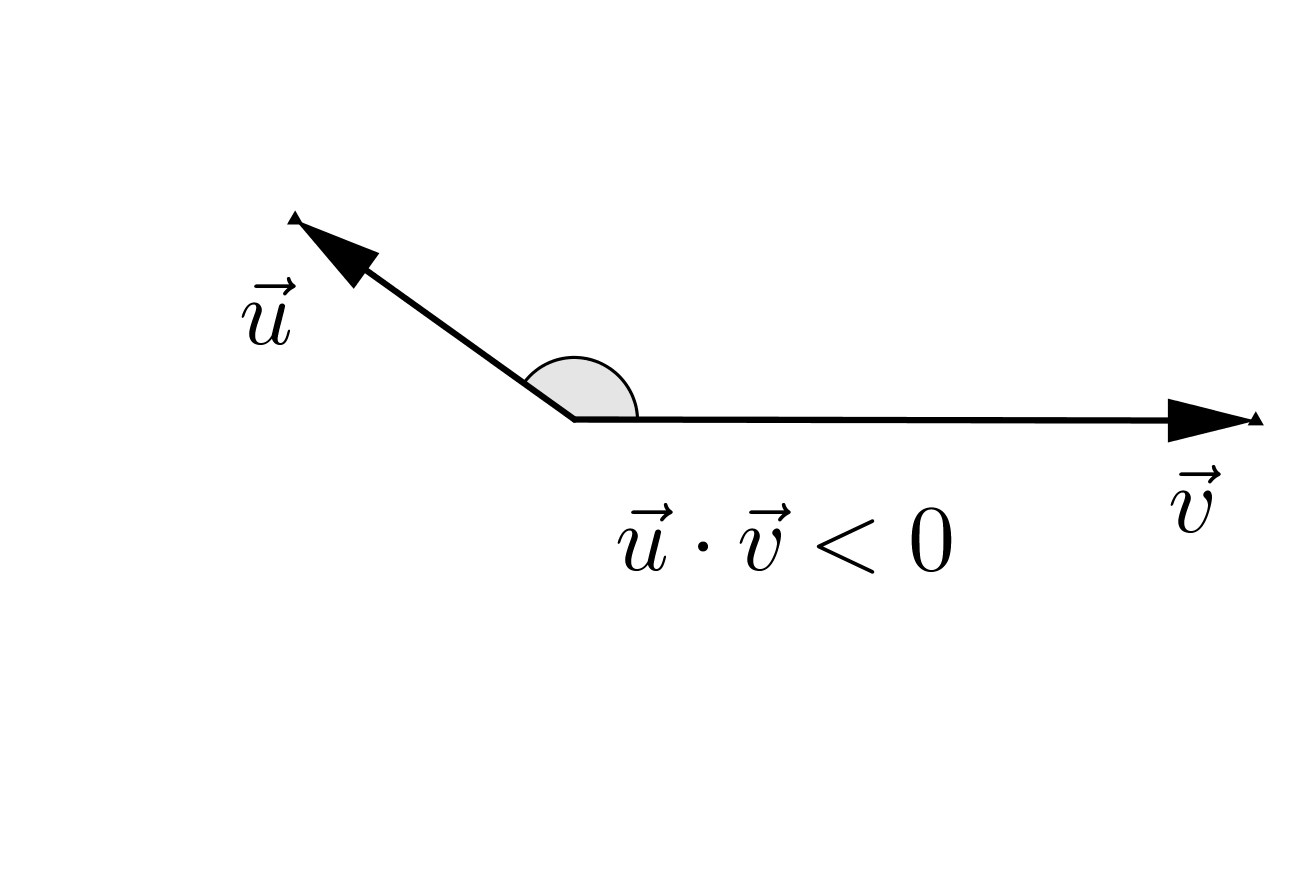
\includegraphics[width=\linewidth]{analitica/imagens/angvetores1.png}
\caption{Ângulo obtuso}
\end{minipage} \hfill
\begin{minipage}[b]{0.3\linewidth}
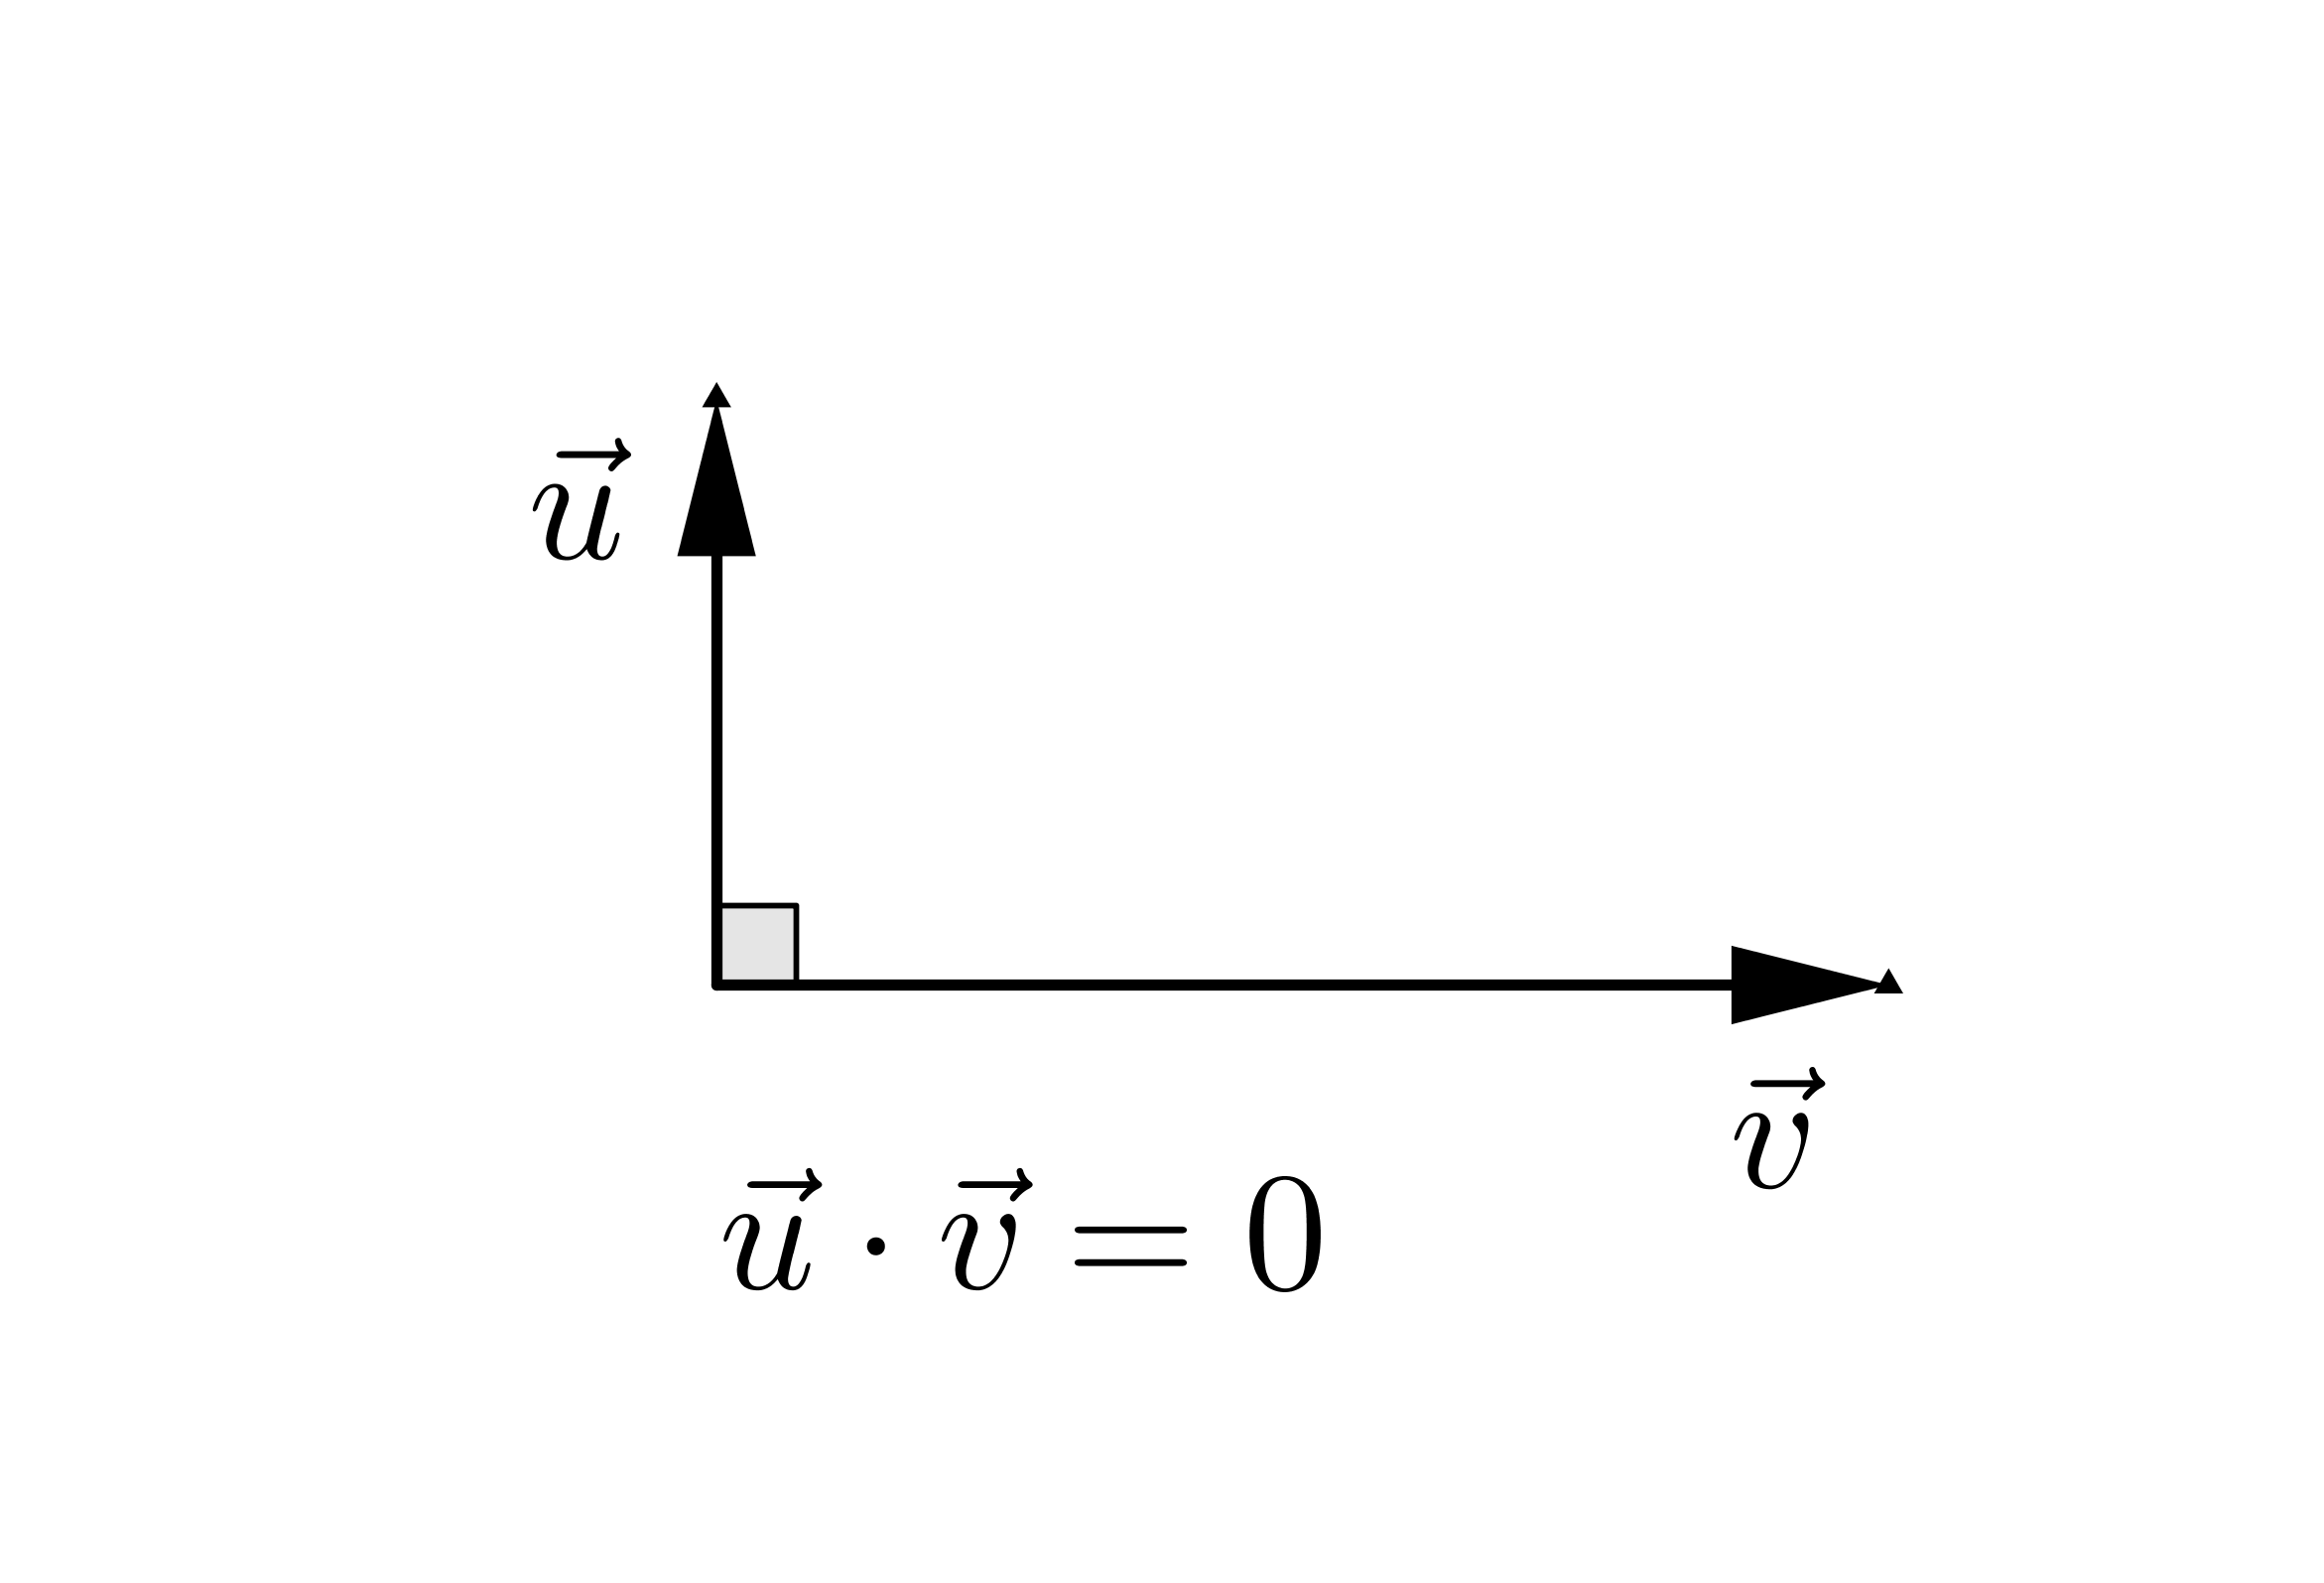
\includegraphics[width=\linewidth]{analitica/imagens/angvetores2.png}
\caption{Ângulo reto}
\end{minipage}\hfill
\begin{minipage}[b]{0.3\linewidth}
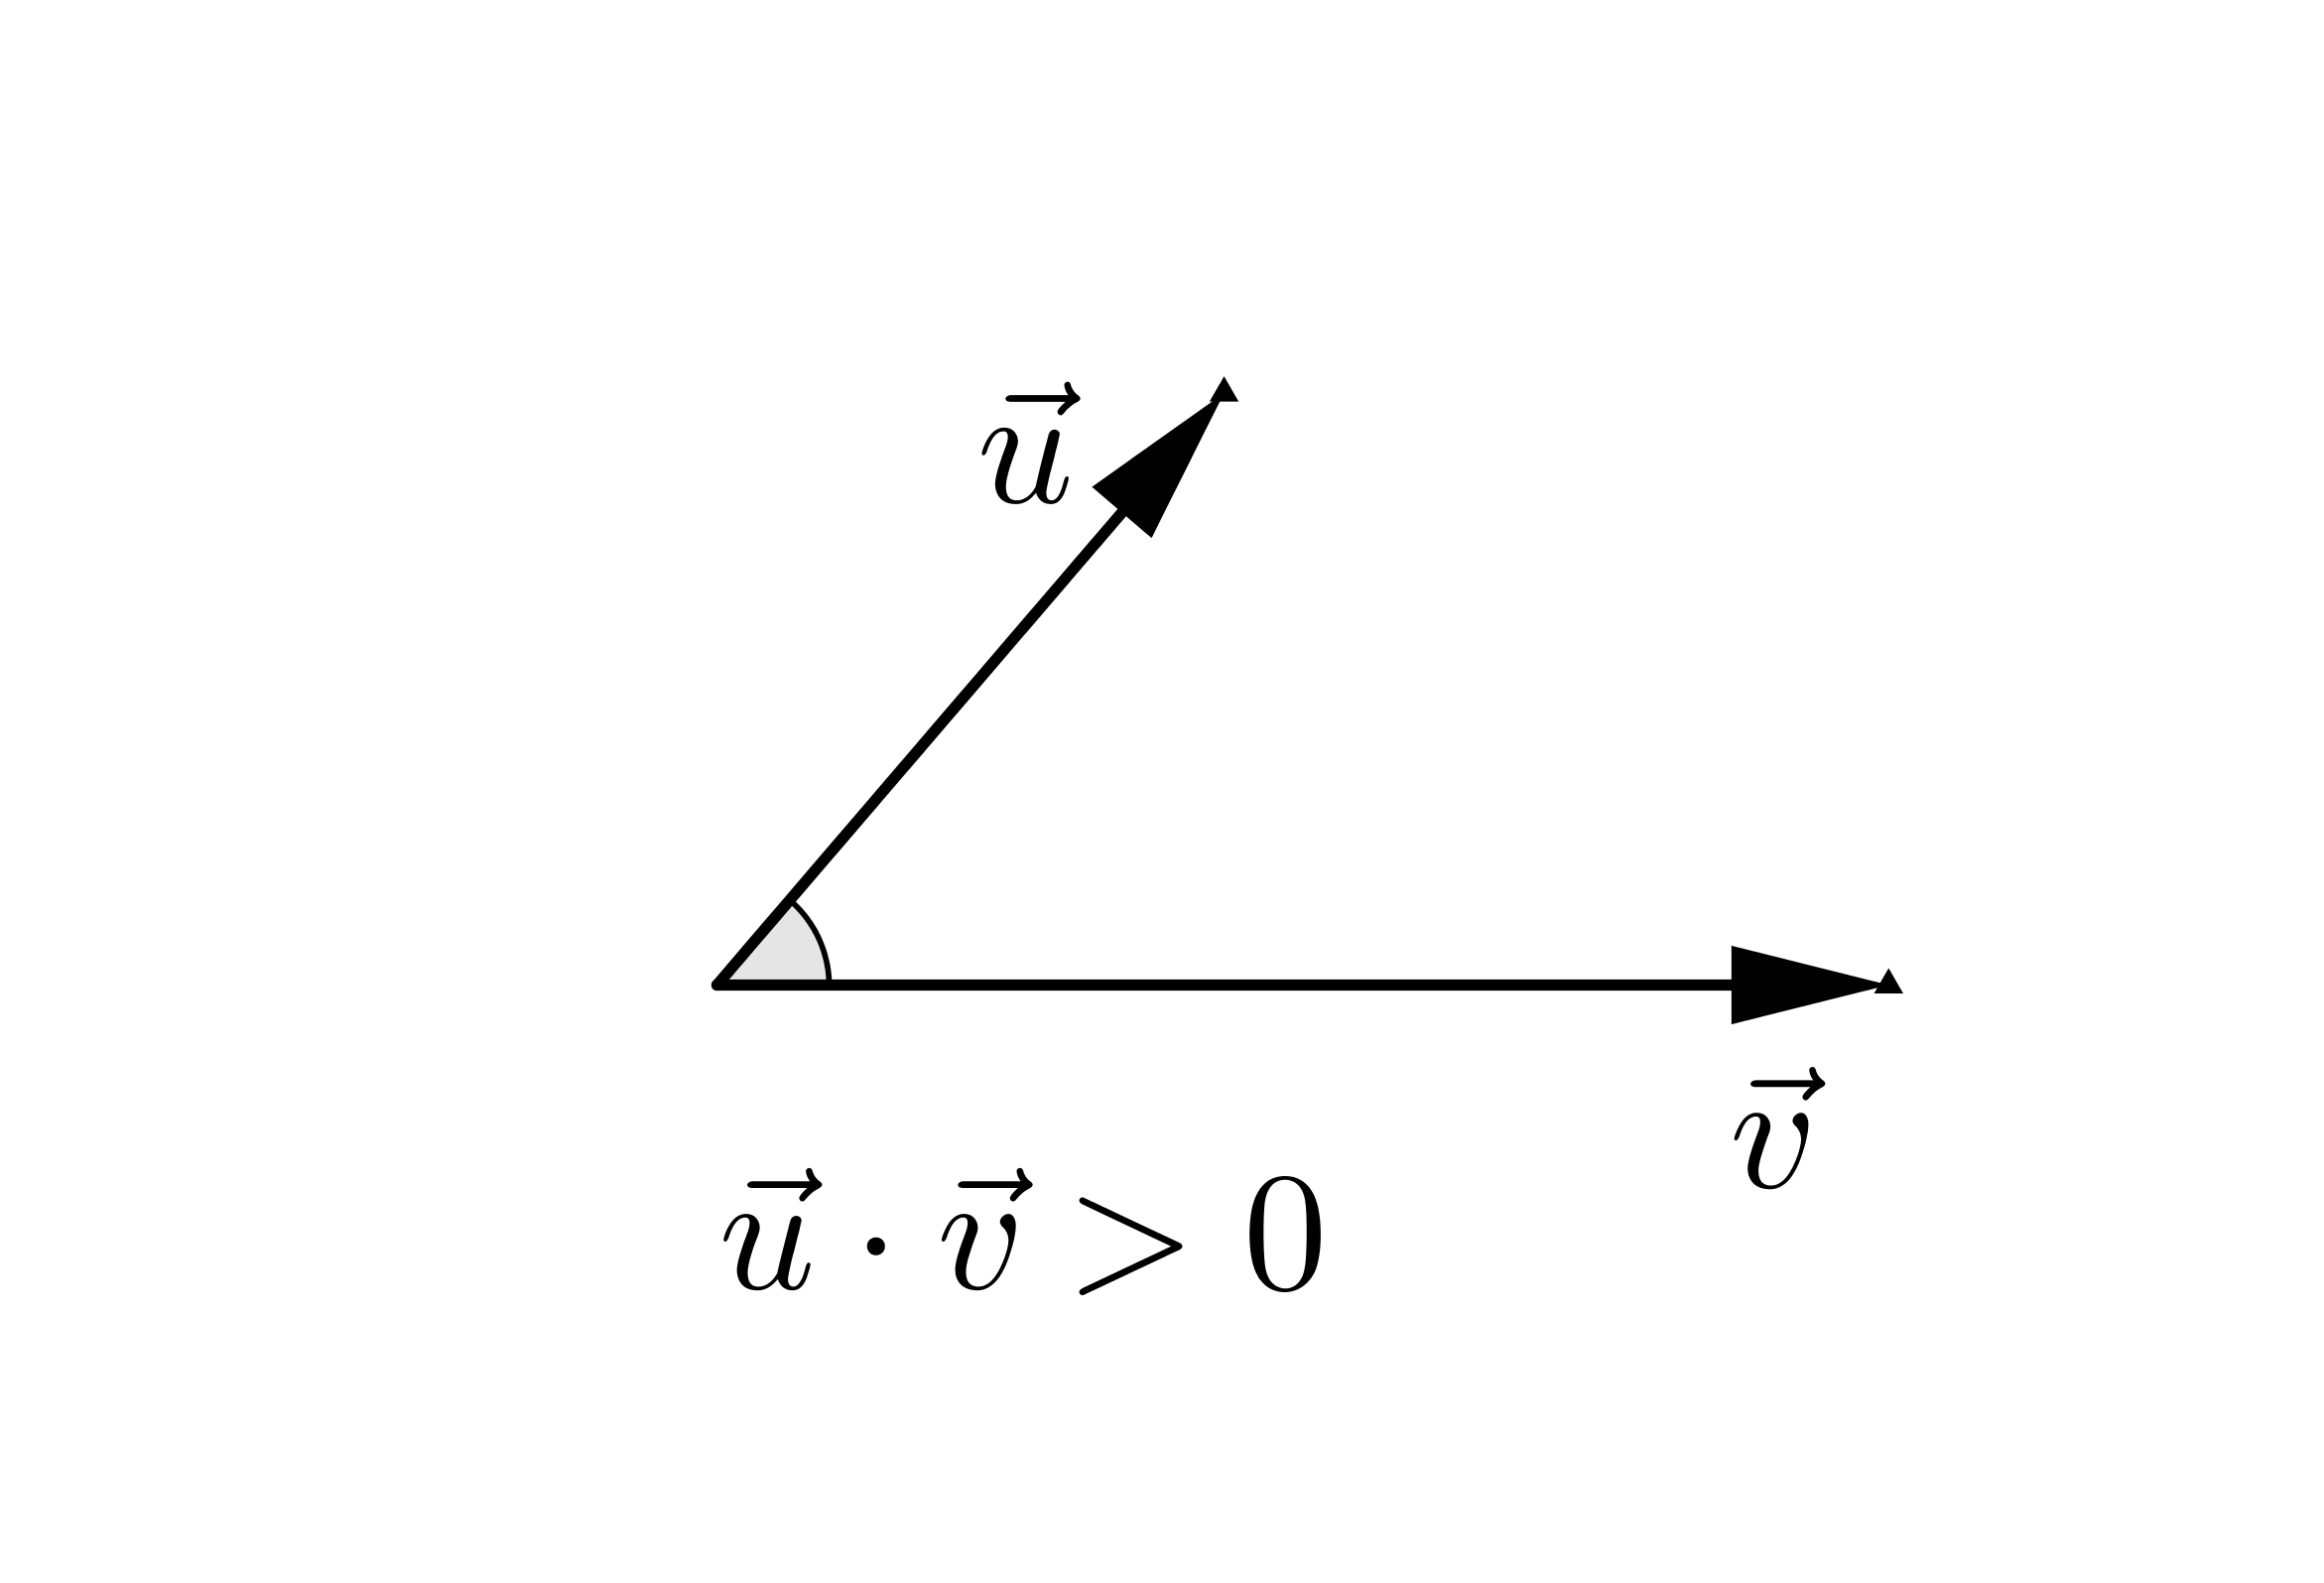
\includegraphics[width=\linewidth]{analitica/imagens/angvetores3.png}
\caption{Ângulo agudo}
\end{minipage}
\end{figure}

\begin{exemplo} dados os vetores $\vec{u}= (4, 3)$ e $\vec{v}=(2,-2)$, determine o cosseno do ângulo formado pelos vetores $\vec{u}$ e $\vec{v}$.
\end{exemplo}

\vspace{2cm}

\begin{exemplo} Qual o ângulo entre os vetores $\vec{u}=(1,-2, 3)$ e $\vec{v}=(4,5,2)$?
\end{exemplo}

\vspace{2cm}

\subsection{Projeção de um vetor sobre outro}

Sejam os vetores $\vec u$ e $\vec v$, pretendemos decompor um dos vetores, digamos $\vec v$, tal que $$\vec v=\vec v_1+\vec v_2$$ sendo $\vec v_1\parallel\vec u$ e $\vec v_2 \perp \vec u$.

\begin{figure}[H]
\centering
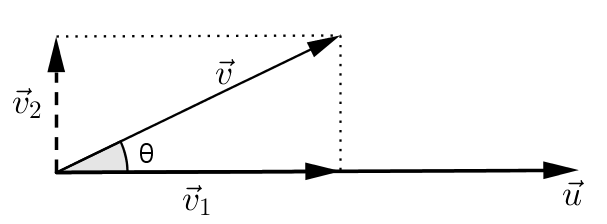
\includegraphics[scale=1]{analitica/imagens/projecao.png}
\end{figure}

O vetor $\vec v_1$ é chamado \textit{projeção ortogonal} de $\vec v$ sobre $\vec u$ e indicado por $$\vec v_1=proj_{\vec u}\vec v$$

\textbf{Demonstração:} Sendo $\vec v_1\parallel \vec u$, temos $\vec v_1=\alpha \vec u$, e como $\vec v_2=\vec v-\vec v_1=\vec v-\alpha\vec u$ é ortogonal a $\vec u$, temos\footnote{Observe que $\alpha$ é uma constante, já que o resultado do produto escalar é um número real.}

\begin{eqnarray*}
(\vec v-\alpha \vec u) \cdot \vec u & = & 0 \\
\vec v \cdot \vec u-\alpha \vec u \cdot \vec u& = &  0\\
\alpha \vec u \cdot \vec u& = &  \vec v \cdot \vec u\\
\alpha & = & \frac{\vec v \cdot \vec u}{\vec u \cdot \vec u}
\end{eqnarray*}

Lembrando que $\vec v_1=\alpha \vec u$, concluímos que  $\vec v_1= \left(\frac{\vec v \cdot \vec u}{\vec u \cdot \vec u}\right) \vec u$.

Portanto, a \textit{projeção ortogonal} de $\vec v$ sobre $\vec u$ é dada por $$proj_{\vec u}\vec v=\left(\frac{\vec v \cdot \vec u}{\vec u \cdot \vec u}\right) \vec u$$